% Bagian Tahapan Percobaan
\section*{Tahapan Percobaan} % Jika ada tahapan percobaan

Dalam modul ini, sebelum melakukan konfigurasi routing statis dan dinamis, terlebih dahulu kita harus menyiapkan topologi yang akan digunakan untuk percobaan 1 dan 2. Topologi yang digunakan ditulis dalam kertas seperti pada Gambar \ref{fig:topo}.

\begin{figure}[H]
    \centering
    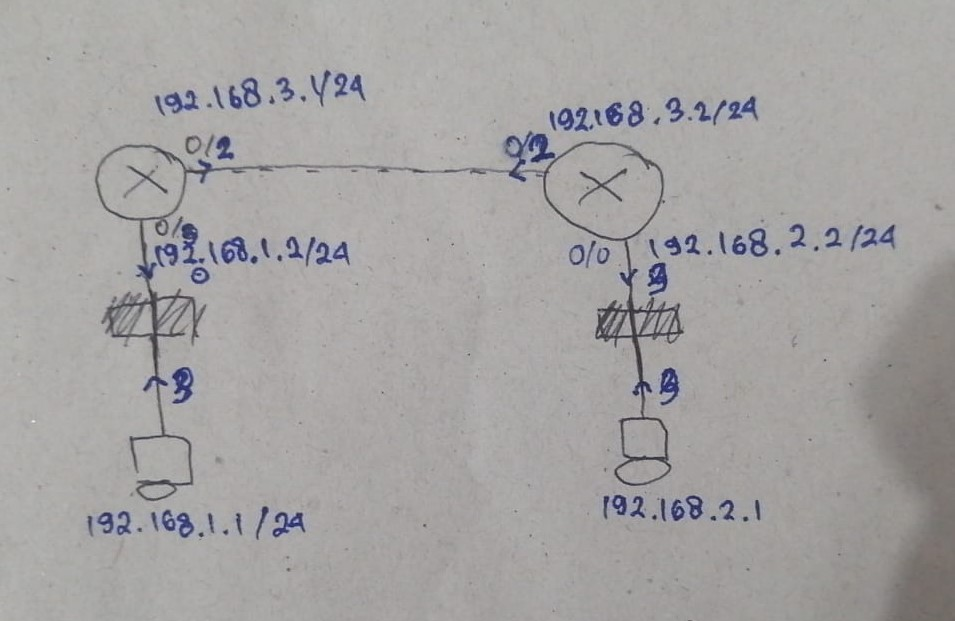
\includegraphics[width=0.8\textwidth]{img/topologi.jpeg}
    \caption{Topologi yang akan digunakan}
    \label{fig:topo}
\end{figure}

Setelah topologi selesai disiapkan, langkah selanjutnya adalah melakukan konfigurasi routing statis dan dinamis pada perangkat MikroTik. Berikut adalah tahapan percobaan yang harus dilakukan:

\subsection*{Percobaan 2: Konfigurasi Dynamic Routing}

\subsubsection*{Konfigurasi Router 1}

\begin{enumerate}
    \item \textbf{Buka WinBox}: Buka aplikasi WinBox dan lakukan koneksi ke Router 1.
    \item \textbf{Atur IP Address}: Berikan IP Address pada interface \texttt{ether} (yang terhubung ke laptop/PC) dan \texttt{ether} (yang terhubung ke Router lain) pada tab \texttt{IP > Addresses}. Pastikan IP Address yang diberikan sesuai dan berbeda dari contoh di modul.
    \item \textbf{Routing Dinamis (RIP)}:
    \begin{enumerate}
        \item Buka tab \texttt{Routing > RIP}.
        \item Pada bagian \texttt{Interfaces}, tambahkan interface baru dan atur interface menjadi \texttt{ether} (yang terhubung ke Router lain).
        \item Pada bagian \texttt{Networks}, tambahkan dua network baru:
        \begin{itemize}
            \item Network antara PC1 dengan Router 1.
            \item Network antara Router 1 dengan Router 2.
        \end{itemize}
        \item Pada bagian \texttt{Neighbours}, tambahkan alamat IP Router 2.
    \end{enumerate}
\end{enumerate}

\subsubsection*{Konfigurasi Router 2}

\begin{enumerate}
    \item \textbf{Buka WinBox}: Buka aplikasi WinBox dan lakukan koneksi ke Router 2.
    \item \textbf{Atur IP Address}: Berikan IP Address pada interface \texttt{ether} (yang terhubung ke laptop/PC) dan \texttt{ether} (yang terhubung ke Router lain) pada tab \texttt{IP > Addresses}. Pastikan IP Address yang diberikan sesuai dan berbeda dari contoh di modul.
    \item \textbf{Routing Dinamis (RIP)}:
    \begin{enumerate}
        \item Buka tab \texttt{Routing > RIP}.
        \item Pada bagian \texttt{Interfaces}, tambahkan interface baru dan atur interface menjadi \texttt{ether} (yang terhubung ke Router lain).
        \item Pada bagian \texttt{Networks}, tambahkan dua network baru:
        \begin{itemize}
            \item Network antara PC2 dengan Router 2.
            \item Network antara Router 1 dengan Router 2.
        \end{itemize}
        \item Pada bagian \texttt{Neighbours}, tambahkan alamat IP Router 1.
    \end{enumerate}
\end{enumerate}

\subsubsection*{Pengujian Konfigurasi}

\begin{enumerate}
    \item \textbf{Ping Router 1 ke Router 2}: Lakukan tes ping dari Router 1 ke Router 2 untuk memastikan konektivitas.
    \item \textbf{Ping Router 2 ke Router 1}: Lakukan tes ping dari Router 2 ke Router 1 untuk memastikan konektivitas.
\end{enumerate}